\documentclass{standalone}
\usepackage{tikz}
\usetikzlibrary{patterns, positioning}


\begin{document}
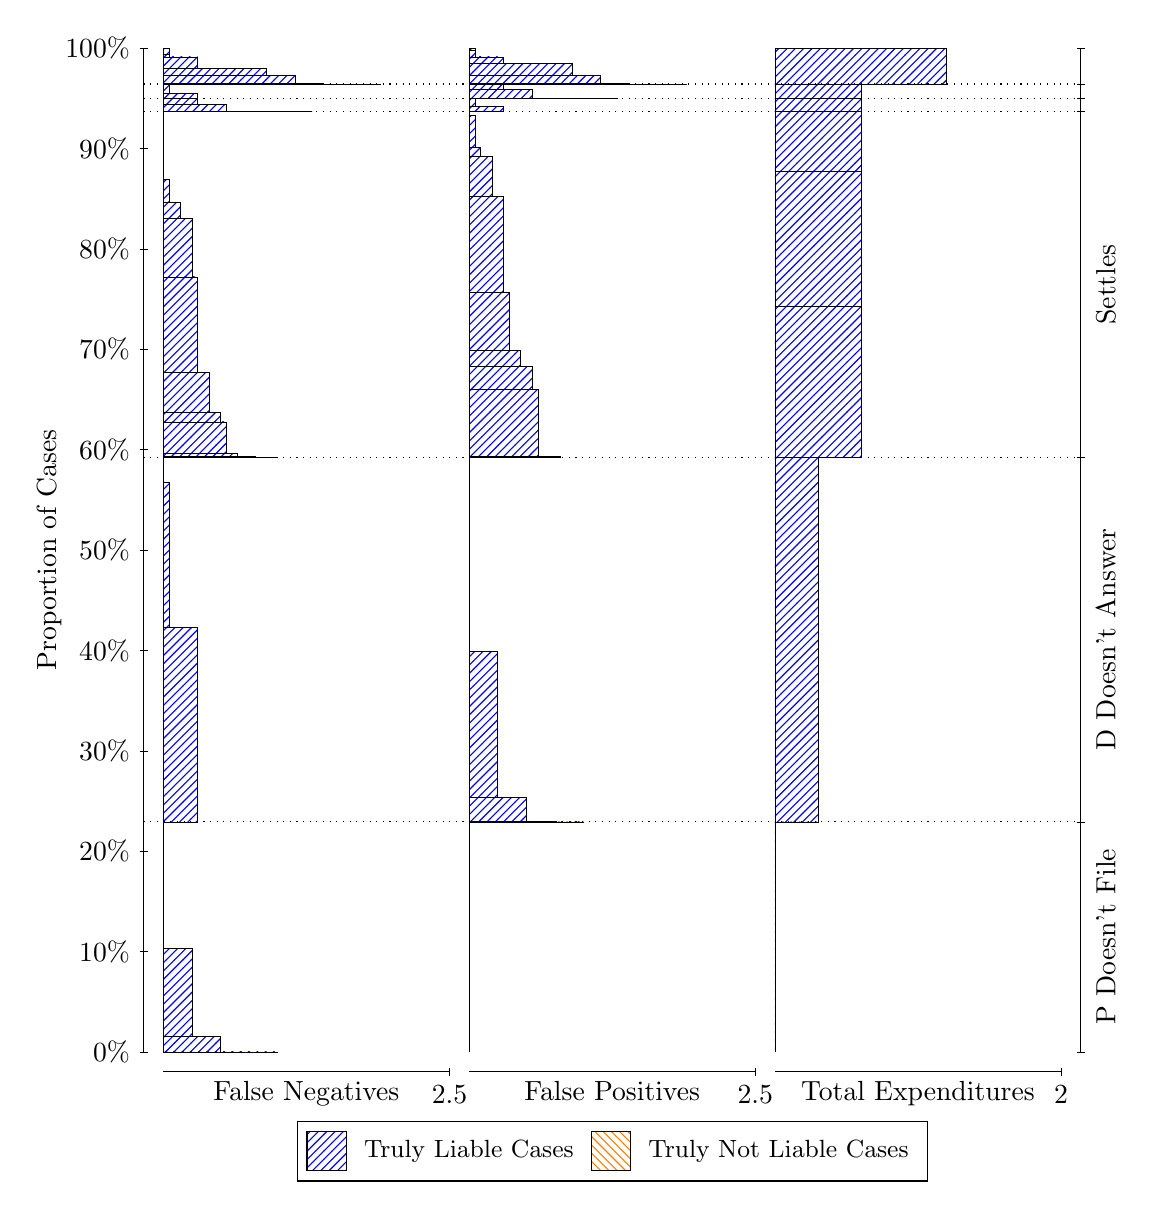
\begin{tikzpicture}
\draw[black, very thin] (1.5,1.75) -- (1.5,14.5);
\node[rotate=90, text=black, anchor=center] at (0.3, 8.125) {Proportion of Cases};
\draw[black, very thin] (1.45,1.75) -- (1.55,1.75);
\node[text=black, anchor=east] at (1.45, 1.75) {0\%};
\draw[black, very thin] (1.45,3.025) -- (1.55,3.025);
\node[text=black, anchor=east] at (1.45, 3.025) {10\%};
\draw[black, very thin] (1.45,4.3) -- (1.55,4.3);
\node[text=black, anchor=east] at (1.45, 4.3) {20\%};
\draw[black, very thin] (1.45,5.575) -- (1.55,5.575);
\node[text=black, anchor=east] at (1.45, 5.575) {30\%};
\draw[black, very thin] (1.45,6.85) -- (1.55,6.85);
\node[text=black, anchor=east] at (1.45, 6.85) {40\%};
\draw[black, very thin] (1.45,8.125) -- (1.55,8.125);
\node[text=black, anchor=east] at (1.45, 8.125) {50\%};
\draw[black, very thin] (1.45,9.4) -- (1.55,9.4);
\node[text=black, anchor=east] at (1.45, 9.4) {60\%};
\draw[black, very thin] (1.45,10.675) -- (1.55,10.675);
\node[text=black, anchor=east] at (1.45, 10.675) {70\%};
\draw[black, very thin] (1.45,11.95) -- (1.55,11.95);
\node[text=black, anchor=east] at (1.45, 11.95) {80\%};
\draw[black, very thin] (1.45,13.225) -- (1.55,13.225);
\node[text=black, anchor=east] at (1.45, 13.225) {90\%};
\draw[black, very thin] (1.45,14.5) -- (1.55,14.5);
\node[text=black, anchor=east] at (1.45, 14.5) {100\%};

\draw[black, very thin] (13.4,1.75) -- (13.4,14.5);
\draw[black, very thin] (13.35,1.75) -- (13.45,1.75);
\node[anchor=west] at (13.35, 1.75) {};
\draw[black, very thin] (13.35,4.6733) -- (13.45,4.6733);
\node[anchor=west] at (13.35, 4.6733) {};
\draw[black, very thin] (13.35,9.3026) -- (13.45,9.3026);
\node[anchor=west] at (13.35, 9.3026) {};
\draw[black, very thin] (13.35,13.691) -- (13.45,13.691);
\node[anchor=west] at (13.35, 13.691) {};
\draw[black, very thin] (13.35,13.859) -- (13.45,13.859);
\node[anchor=west] at (13.35, 13.859) {};
\draw[black, very thin] (13.35,14.043) -- (13.45,14.043);
\node[anchor=west] at (13.35, 14.043) {};
\draw[black, very thin] (13.35,14.5) -- (13.45,14.5);
\node[anchor=west] at (13.35, 14.5) {};

\draw[black, very thin, pattern color=blue, pattern=north east lines] (1.75,1.75) rectangle (3.2033,1.75);
\draw[black, very thin, pattern color=blue, pattern=north east lines] (1.75,1.75) rectangle (2.84,1.7517);
\draw[black, very thin, pattern color=blue, pattern=north east lines] (1.75,1.7517) rectangle (2.4767,1.9487);
\draw[black, very thin, pattern color=blue, pattern=north east lines] (1.75,1.9487) rectangle (2.1133,3.0625);
\draw[black, very thin, pattern color=orange, pattern=north west lines] (1.75,3.0625) rectangle (1.75,3.0625);
\draw[black, very thin, pattern color=blue, pattern=north east lines] (1.75,3.0625) rectangle (1.75,4.6733);
\draw[black, very thin, pattern color=blue, pattern=north east lines] (1.75,4.6733) rectangle (2.186,7.139);
\draw[black, very thin, pattern color=blue, pattern=north east lines] (1.75,7.139) rectangle (1.8227,8.9896);
\draw[black, very thin, pattern color=orange, pattern=north west lines] (1.75,8.9896) rectangle (1.75,8.9896);
\draw[black, very thin, pattern color=blue, pattern=north east lines] (1.75,8.9896) rectangle (1.75,9.3026);
\draw[black, very thin, pattern color=blue, pattern=north east lines] (1.75,9.3026) rectangle (3.2033,9.3026);
\draw[black, very thin, pattern color=blue, pattern=north east lines] (1.75,9.3026) rectangle (3.058,9.3026);
\draw[black, very thin, pattern color=blue, pattern=north east lines] (1.75,9.3026) rectangle (2.9127,9.3137);
\draw[black, very thin, pattern color=blue, pattern=north east lines] (1.75,9.3137) rectangle (2.84,9.3142);
\draw[black, very thin, pattern color=blue, pattern=north east lines] (1.75,9.3142) rectangle (2.6947,9.3479);
\draw[black, very thin, pattern color=blue, pattern=north east lines] (1.75,9.3479) rectangle (2.5493,9.7528);
\draw[black, very thin, pattern color=blue, pattern=north east lines] (1.75,9.7528) rectangle (2.4767,9.8736);
\draw[black, very thin, pattern color=blue, pattern=north east lines] (1.75,9.8736) rectangle (2.3313,10.383);
\draw[black, very thin, pattern color=blue, pattern=north east lines] (1.75,10.383) rectangle (2.186,11.593);
\draw[black, very thin, pattern color=blue, pattern=north east lines] (1.75,11.593) rectangle (2.1133,12.335);
\draw[black, very thin, pattern color=blue, pattern=north east lines] (1.75,12.335) rectangle (1.968,12.539);
\draw[black, very thin, pattern color=blue, pattern=north east lines] (1.75,12.539) rectangle (1.8227,12.827);
\draw[black, very thin, pattern color=orange, pattern=north west lines] (1.75,12.827) rectangle (1.75,12.827);
\draw[black, very thin, pattern color=blue, pattern=north east lines] (1.75,12.827) rectangle (1.75,13.691);
\draw[black, very thin, pattern color=blue, pattern=north east lines] (1.75,13.691) rectangle (3.6393,13.691);
\draw[black, very thin, pattern color=blue, pattern=north east lines] (1.75,13.691) rectangle (3.276,13.691);
\draw[black, very thin, pattern color=blue, pattern=north east lines] (1.75,13.691) rectangle (2.9127,13.694);
\draw[black, very thin, pattern color=blue, pattern=north east lines] (1.75,13.694) rectangle (2.5493,13.787);
\draw[black, very thin, pattern color=blue, pattern=north east lines] (1.75,13.787) rectangle (2.186,13.859);
\draw[black, very thin, pattern color=orange, pattern=north west lines] (1.75,13.859) rectangle (1.75,13.859);
\draw[black, very thin, pattern color=blue, pattern=north east lines] (1.75,13.859) rectangle (2.186,13.928);
\draw[black, very thin, pattern color=blue, pattern=north east lines] (1.75,13.928) rectangle (1.8227,14.038);
\draw[black, very thin, pattern color=orange, pattern=north west lines] (1.75,14.038) rectangle (1.75,14.038);
\draw[black, very thin, pattern color=blue, pattern=north east lines] (1.75,14.038) rectangle (1.75,14.043);
\draw[black, very thin, pattern color=blue, pattern=north east lines] (1.75,14.043) rectangle (4.5113,14.043);
\draw[black, very thin, pattern color=blue, pattern=north east lines] (1.75,14.043) rectangle (4.148,14.043);
\draw[black, very thin, pattern color=blue, pattern=north east lines] (1.75,14.043) rectangle (3.7847,14.051);
\draw[black, very thin, pattern color=blue, pattern=north east lines] (1.75,14.051) rectangle (3.4213,14.155);
\draw[black, very thin, pattern color=blue, pattern=north east lines] (1.75,14.155) rectangle (3.276,14.155);
\draw[black, very thin, pattern color=blue, pattern=north east lines] (1.75,14.155) rectangle (3.058,14.238);
\draw[black, very thin, pattern color=blue, pattern=north east lines] (1.75,14.238) rectangle (2.9127,14.238);
\draw[black, very thin, pattern color=blue, pattern=north east lines] (1.75,14.238) rectangle (2.6947,14.238);
\draw[black, very thin, pattern color=blue, pattern=north east lines] (1.75,14.238) rectangle (2.5493,14.24);
\draw[black, very thin, pattern color=blue, pattern=north east lines] (1.75,14.24) rectangle (2.3313,14.24);
\draw[black, very thin, pattern color=blue, pattern=north east lines] (1.75,14.24) rectangle (2.186,14.242);
\draw[black, very thin, pattern color=blue, pattern=north east lines] (1.75,14.242) rectangle (2.186,14.387);
\draw[black, very thin, pattern color=blue, pattern=north east lines] (1.75,14.387) rectangle (1.8227,14.423);
\draw[black, very thin, pattern color=blue, pattern=north east lines] (1.75,14.423) rectangle (1.8227,14.493);
\draw[black, very thin, pattern color=orange, pattern=north west lines] (1.75,14.493) rectangle (1.75,14.493);
\draw[black, very thin, pattern color=blue, pattern=north east lines] (1.75,14.493) rectangle (1.75,14.5);
\draw[black, very thin, pattern color=orange, pattern=north west lines] (5.6333,1.75) rectangle (5.6333,1.75);
\draw[black, very thin, pattern color=blue, pattern=north east lines] (5.6333,1.75) rectangle (5.6333,4.6733);
\draw[black, very thin, pattern color=orange, pattern=north west lines] (5.6333,4.6733) rectangle (7.0867,4.6733);
\draw[black, very thin, pattern color=blue, pattern=north east lines] (5.6333,4.6733) rectangle (7.0867,4.6733);
\draw[black, very thin, pattern color=blue, pattern=north east lines] (5.6333,4.6733) rectangle (6.7233,4.675);
\draw[black, very thin, pattern color=blue, pattern=north east lines] (5.6333,4.675) rectangle (6.36,4.9864);
\draw[black, very thin, pattern color=blue, pattern=north east lines] (5.6333,4.9864) rectangle (5.9967,6.8369);
\draw[black, very thin, pattern color=blue, pattern=north east lines] (5.6333,6.8369) rectangle (5.6333,9.3026);
\draw[black, very thin, pattern color=orange, pattern=north west lines] (5.6333,9.3026) rectangle (6.796,9.3026);
\draw[black, very thin, pattern color=blue, pattern=north east lines] (5.6333,9.3026) rectangle (6.796,9.3098);
\draw[black, very thin, pattern color=orange, pattern=north west lines] (5.6333,9.3098) rectangle (6.6507,9.3098);
\draw[black, very thin, pattern color=blue, pattern=north east lines] (5.6333,9.3098) rectangle (6.6507,9.3152);
\draw[black, very thin, pattern color=orange, pattern=north west lines] (5.6333,9.3152) rectangle (6.5053,9.3152);
\draw[black, very thin, pattern color=blue, pattern=north east lines] (5.6333,9.3152) rectangle (6.5053,10.168);
\draw[black, very thin, pattern color=blue, pattern=north east lines] (5.6333,10.168) rectangle (6.4327,10.455);
\draw[black, very thin, pattern color=blue, pattern=north east lines] (5.6333,10.455) rectangle (6.2873,10.66);
\draw[black, very thin, pattern color=blue, pattern=north east lines] (5.6333,10.66) rectangle (6.142,11.401);
\draw[black, very thin, pattern color=blue, pattern=north east lines] (5.6333,11.401) rectangle (6.0693,12.611);
\draw[black, very thin, pattern color=blue, pattern=north east lines] (5.6333,12.611) rectangle (5.924,13.12);
\draw[black, very thin, pattern color=blue, pattern=north east lines] (5.6333,13.12) rectangle (5.7787,13.241);
\draw[black, very thin, pattern color=blue, pattern=north east lines] (5.6333,13.241) rectangle (5.706,13.646);
\draw[black, very thin, pattern color=blue, pattern=north east lines] (5.6333,13.646) rectangle (5.6333,13.691);
\draw[black, very thin, pattern color=orange, pattern=north west lines] (5.6333,13.691) rectangle (6.0693,13.691);
\draw[black, very thin, pattern color=blue, pattern=north east lines] (5.6333,13.691) rectangle (6.0693,13.763);
\draw[black, very thin, pattern color=blue, pattern=north east lines] (5.6333,13.763) rectangle (5.706,13.856);
\draw[black, very thin, pattern color=blue, pattern=north east lines] (5.6333,13.856) rectangle (5.6333,13.859);
\draw[black, very thin, pattern color=orange, pattern=north west lines] (5.6333,13.859) rectangle (7.5227,13.859);
\draw[black, very thin, pattern color=blue, pattern=north east lines] (5.6333,13.859) rectangle (7.5227,13.859);
\draw[black, very thin, pattern color=blue, pattern=north east lines] (5.6333,13.859) rectangle (7.1593,13.859);
\draw[black, very thin, pattern color=blue, pattern=north east lines] (5.6333,13.859) rectangle (6.796,13.864);
\draw[black, very thin, pattern color=blue, pattern=north east lines] (5.6333,13.864) rectangle (6.4327,13.973);
\draw[black, very thin, pattern color=blue, pattern=north east lines] (5.6333,13.973) rectangle (6.0693,14.043);
\draw[black, very thin, pattern color=orange, pattern=north west lines] (5.6333,14.043) rectangle (8.3947,14.043);
\draw[black, very thin, pattern color=blue, pattern=north east lines] (5.6333,14.043) rectangle (8.3947,14.043);
\draw[black, very thin, pattern color=orange, pattern=north west lines] (5.6333,14.043) rectangle (8.0313,14.043);
\draw[black, very thin, pattern color=blue, pattern=north east lines] (5.6333,14.043) rectangle (8.0313,14.043);
\draw[black, very thin, pattern color=orange, pattern=north west lines] (5.6333,14.043) rectangle (7.668,14.043);
\draw[black, very thin, pattern color=blue, pattern=north east lines] (5.6333,14.043) rectangle (7.668,14.05);
\draw[black, very thin, pattern color=orange, pattern=north west lines] (5.6333,14.05) rectangle (7.3047,14.05);
\draw[black, very thin, pattern color=blue, pattern=north east lines] (5.6333,14.05) rectangle (7.3047,14.155);
\draw[black, very thin, pattern color=blue, pattern=north east lines] (5.6333,14.155) rectangle (6.9413,14.303);
\draw[black, very thin, pattern color=orange, pattern=north west lines] (5.6333,14.303) rectangle (6.796,14.303);
\draw[black, very thin, pattern color=blue, pattern=north east lines] (5.6333,14.303) rectangle (6.796,14.303);
\draw[black, very thin, pattern color=blue, pattern=north east lines] (5.6333,14.303) rectangle (6.578,14.305);
\draw[black, very thin, pattern color=orange, pattern=north west lines] (5.6333,14.305) rectangle (6.4327,14.305);
\draw[black, very thin, pattern color=blue, pattern=north east lines] (5.6333,14.305) rectangle (6.4327,14.305);
\draw[black, very thin, pattern color=blue, pattern=north east lines] (5.6333,14.305) rectangle (6.2147,14.305);
\draw[black, very thin, pattern color=blue, pattern=north east lines] (5.6333,14.305) rectangle (6.0693,14.386);
\draw[black, very thin, pattern color=orange, pattern=north west lines] (5.6333,14.386) rectangle (6.0693,14.386);
\draw[black, very thin, pattern color=blue, pattern=north east lines] (5.6333,14.386) rectangle (6.0693,14.388);
\draw[black, very thin, pattern color=blue, pattern=north east lines] (5.6333,14.388) rectangle (5.8513,14.388);
\draw[black, very thin, pattern color=blue, pattern=north east lines] (5.6333,14.388) rectangle (5.706,14.467);
\draw[black, very thin, pattern color=blue, pattern=north east lines] (5.6333,14.467) rectangle (5.706,14.492);
\draw[black, very thin, pattern color=blue, pattern=north east lines] (5.6333,14.492) rectangle (5.6333,14.5);
\draw[black, very thin, pattern color=orange, pattern=north west lines] (9.5167,1.75) rectangle (9.5167,1.75);
\draw[black, very thin, pattern color=blue, pattern=north east lines] (9.5167,1.75) rectangle (9.5167,4.6733);
\draw[black, very thin, pattern color=orange, pattern=north west lines] (9.5167,4.6733) rectangle (10.062,4.6733);
\draw[black, very thin, pattern color=blue, pattern=north east lines] (9.5167,4.6733) rectangle (10.062,9.3026);
\draw[black, very thin, pattern color=orange, pattern=north west lines] (9.5167,9.3026) rectangle (10.607,9.3026);
\draw[black, very thin, pattern color=blue, pattern=north east lines] (9.5167,9.3026) rectangle (10.607,11.222);
\draw[black, very thin, pattern color=orange, pattern=north west lines] (9.5167,11.222) rectangle (10.607,11.222);
\draw[black, very thin, pattern color=blue, pattern=north east lines] (9.5167,11.222) rectangle (10.607,12.938);
\draw[black, very thin, pattern color=orange, pattern=north west lines] (9.5167,12.938) rectangle (10.607,12.938);
\draw[black, very thin, pattern color=blue, pattern=north east lines] (9.5167,12.938) rectangle (10.607,13.691);
\draw[black, very thin, pattern color=orange, pattern=north west lines] (9.5167,13.691) rectangle (10.607,13.691);
\draw[black, very thin, pattern color=blue, pattern=north east lines] (9.5167,13.691) rectangle (10.607,13.859);
\draw[black, very thin, pattern color=orange, pattern=north west lines] (9.5167,13.859) rectangle (10.607,13.859);
\draw[black, very thin, pattern color=blue, pattern=north east lines] (9.5167,13.859) rectangle (10.607,14.043);
\draw[black, very thin, pattern color=orange, pattern=north west lines] (9.5167,14.043) rectangle (11.697,14.043);
\draw[black, very thin, pattern color=blue, pattern=north east lines] (9.5167,14.043) rectangle (11.697,14.5);
\draw[black, dotted] (1.5,4.6733) -- (13.4,4.6733);
\draw[black, dotted] (1.5,9.3026) -- (13.4,9.3026);
\draw[black, dotted] (1.5,13.691) -- (13.4,13.691);
\draw[black, dotted] (1.5,13.859) -- (13.4,13.859);
\draw[black, dotted] (1.5,14.043) -- (13.4,14.043);
\draw[black, very thin] (1.75,1.5) -- (5.3833,1.5);
\node[text=black, anchor=north] at (3.5667, 1.5) {False Negatives};
\draw[black, very thin] (5.3833,1.45) -- (5.3833,1.55);
\node[text=black, anchor=north] at (5.3833, 1.45) {2.5};

\draw[black, very thin] (5.6333,1.5) -- (9.2667,1.5);
\node[text=black, anchor=north] at (7.45, 1.5) {False Positives};
\draw[black, very thin] (9.2667,1.45) -- (9.2667,1.55);
\node[text=black, anchor=north] at (9.2667, 1.45) {2.5};

\draw[black, very thin] (9.5167,1.5) -- (13.15,1.5);
\node[text=black, anchor=north] at (11.333, 1.5) {Total Expenditures};
\draw[black, very thin] (13.15,1.45) -- (13.15,1.55);
\node[text=black, anchor=north] at (13.15, 1.45) {2};

\node[text=black, centered, rotate=90] at (13.72, 3.2117) {P Doesn't File};
\node[text=black, centered, rotate=90] at (13.72, 6.988) {D Doesn't Answer};
\node[text=black, centered, rotate=90] at (13.72, 11.497) {Settles};




\draw (7.449999999999999,1.5) node[draw=none] (baseCoordinate) {};
\begin{scope}[align=center]
        \matrix[scale=0.5, draw=black, below=0.5cm of baseCoordinate, nodes={draw}, column sep=0.1cm]{
            \node[rectangle, draw, minimum width=0.5cm, minimum height=0.5cm, pattern color=blue, pattern=north east lines] {}; &
            \node[draw=none, font=\small, text=black] (B) {Truly Liable Cases}; &
            \node[rectangle, draw, minimum width=0.5cm, minimum height=0.5cm, pattern color=orange, pattern=north west lines] {}; &
            \node[draw=none, font=\small, text=black] (B) {Truly Not Liable Cases}; \\
            };
\end{scope}

\end{tikzpicture}
\end{document}